\documentclass[fleqn]{article}

\usepackage{amsmath,amssymb,amsthm}
\usepackage{upquote}
\usepackage{hyperref}
\usepackage{tikz}
\usepackage{forest}
\usepackage{geometry}
\usepackage{tabto}
\usetikzlibrary{graphs}

% shortcuts for things commonly used in our class:
\newcommand{\code}{\texttt}
\newcommand{\nat}{\mathbb{N}}
\newcommand{\real}{\mathbb{R}}
\newcommand{\realp}{\mathbb{R}^+}
\newcommand{\bigo}[1]{\mathcal{O}(#1)}
\newcommand{\ital}{\itshape{}}

% command to allow page breaks in align and similar environments
\newcommand{\br}{\displaybreak[0] \\}

% character in a cirle, good to refer to nodes
\newcommand*\circled[1]{\tikz[baseline=(char.base)]{
            \node[shape=circle,draw,inner sep=2pt] (char) {#1};}}
\title{CSCB63 Assignment 1 -- AVL Trees}
\author{***}
\date{Due: February 9th, 2024}
\pagestyle{plain}

\begin{document}
\maketitle

\subsection*{Question 1}

a) \\ 
Let {\itshape f}, {\itshape g}, {\itshape h} : $\mathbb{N} \rightarrow \mathbb{R^+}$.
Suppose {\itshape f} $\in \bigo{g}$, {\itshape g} $\in \bigo{h}$. \\

\noindent $\because$ 
{\itshape f}(n) $\leq$ c$_{1}$ $\cdot$ {\itshape g}(n),
{\itshape g}({\itshape n}) $\leq$ c$_{2}$ $\cdot$ {\ital h}({\itshape n}), 
for some c$_{1}$, c$_{2}$ $\in \mathbb{R^{+}}$. [def. of $\mathcal{O}$]

\noindent $\therefore$
{\ital f}(n) $\leq$ c$_1$ 
$\cdot$ {\ital g}({\ital n}) $\leq$ $c_1$ $\cdot$ c$_2$ $\cdot$ {\ital h}({\ital n}).
[combining inequalities] \\

\noindent
Let c = $c_1 \cdot c_2$. 
$\implies$ {\ital f}(n) $\leq$ c $\cdot$ {\ital h}(n). \\
Hence, {\ital f} $\in \bigo{h}$, as wanted. $\Box$ \\ \\

\noindent
b) \\
Let {\itshape $f_1$}, {\itshape $f_2$}, {\itshape $g_1$}, {\itshape $g_2$} : 
$\mathbb{N} \rightarrow \mathbb{R^+}$.
Suppose {\itshape $f_1$} $\in \bigo{g_1}$, {\itshape $f_2$} $\in \bigo{g_2}$. \\

\noindent $\because$ 
{\itshape f$_1$}({\ital n}) $\leq$ c$_{1}$ $\cdot$ {\itshape g}({\ital n}),
{\itshape f$_2$}({\ital n}) $\leq$ c$_{2}$ $\cdot$ {\itshape g}({\ital n}),
for some c$_{1}$, c$_{2}$ $\in \mathbb{R^{+}}$. [def. of $\mathcal{O}$]

\noindent $\therefore$
{\ital f}({\ital n}) = f$_{1}$({\ital n}) $\cdot$ f$_{2}$({\ital n}) $\leq$
$c_1$ $\cdot$ c$_2$ $\cdot$ {\ital g$_1$}({\ital n}) $\cdot$ {\ital g$_2$}({\ital n}) =
$c_1$ $\cdot$ c$_2$ $\cdot$ {\ital g}({\ital n}).
[combining inequalities] \\

\noindent
Let c = $c_1 \cdot c_2$. 
$\implies$ {\ital f}(n) $\leq$ c $\cdot$ {\ital g}(n). \\
Hence, {\ital f} $\in \bigo{g}$, as wanted. $\Box$ \\ \\

\noindent
c) \\
BWOC, suppose $2^{2n}$ $\in$ $\bigo{2^n}$. \\
Let n = $\lceil{log_2{c}}\rceil$ + 1 $\in$ $\mathbb{N}$. \\

\noindent $\therefore$
c $\cdot$ $2^n$ $\geq$ $2^{2n}$ $\Leftrightarrow$ 
$\log_2{c}$ + n $\geq$ 2n $\Leftrightarrow$
$\log_2{c}$ $\geq$ n = $\lceil{log_2{c}}\rceil$ + 1.
[Contradiction!] \\

\noindent
Hence, $2^{2n}$ $\notin$ $\bigo{2^n}$, as wanted. $\Box$ \pagebreak

\noindent
d) \\
Let {\itshape $f_1$}, {\itshape $f_2$}, {\itshape g} : 
$\mathbb{N} \rightarrow \mathbb{R^+}$.
Suppose {\itshape $f_1$}, {\itshape $f_2$} $\in \bigo{g}$. \\

\noindent $\because$ 
{\itshape f$_1$}({\ital n}) $\leq$ c$_{1}$ $\cdot$ {\itshape g}({\ital n}),
{\itshape f$_2$}({\ital n}) $\leq$ c$_{2}$ $\cdot$ {\itshape g}({\ital n}),
for some c$_{1}$, c$_{2}$ $\in \mathbb{R^{+}}$. [def. of $\mathcal{O}$] \\

\noindent
WLOG, suppose $f_{max}$ = max($f_1$, $f_2$) = $f_1$. \\

\noindent $\therefore$
{\ital f$_{max}$}({\ital n}) = f$_{1}$({\ital n}) $\leq$
$c_1$ $\cdot$ {\ital g}({\ital n}).
[by assumption] \\

\noindent
Let c = $c_1$.
$\implies$ {\ital $f_{max}$}(n) $\leq$ c $\cdot$ {\ital g}(n). \\
Hence, {\ital f} $\in \bigo{g}$, as wanted. $\Box$ \pagebreak

\subsection*{Question 2}

Inserting (9) \\

\begin{center}
    
\begin{tikzpicture}
      \draw[level distance=15mm, level/.style={sibling distance=20mm}, every node/.style={circle,draw},
            edge from parent/.style={-latex,draw}, font=\rmfamily]
      node{9};
    \end{tikzpicture}
\end{center}

\noindent
Inserting (10) \\

\begin{center}
    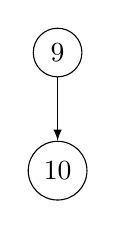
\begin{tikzpicture}
      \draw[level distance=15mm, level/.style={sibling distance=20mm}, every node/.style={circle,draw},
            edge from parent/.style={-latex,draw}, font=\rmfamily]
      node{9}
        child{node{10}
        child[missing]
      };
    \end{tikzpicture}
\end{center}

\end{document}